\chapter{Background Research}\label{ch:background}

This chapter provides the necessary foundation for designing and implementing a liquid democracy system within vodle. It begins by comparing liquid democracy to traditional models (direct and representative democracy) highlighting its potential to balance participation and scalability through transitive and revocable delegation.

The chapter then examines key limitations of liquid democracy in practice, including delegation cycles, abstentions, and the emergence of super-voters. These issues are explored in detail, alongside the strategies proposed in the literature to mitigate them.

Additionally, real-world deployments of liquid democracy are considered, drawing lessons from systems such as LiquidFeedback and Google Votes. These examples inform both the technical feasibility and design challenges of integrating delegation mechanisms into online platforms.

Finally, the chapter outlines the technical foundations of vodle, including its architecture and existing (incomplete) delegation features. These constraints play a key role in shaping the design choices presented in later chapters.

\section{Liquid Democracy}

While liquid democracy was briefly introduced in Chapter~\ref{ch:introduction}, this section provides a more detailed rationale for its relevance -- particularly in the context of decision-making systems like vodle.

\textbf{Direct democracy} maximises personal agency and transparency by allowing individuals to vote on every issue. It is often viewed as the most egalitarian form of governance, as it ensures that all participants have a direct say in decisions. However, it becomes impractical at scale. Expecting all users to remain consistently informed and engaged across all issues is unrealistic, particularly in large or heterogeneous groups \citep{ford_delegative_2002}. As \citeauthor{ford_delegative_2002} observes, the assumption that the majority can or will make consistently well-informed decisions across a broad range of topics does not hold in practice. This can lead to voter fatigue, low turnout, and uninformed or irrational decision-making.

\textbf{Representative democracy} addresses the scalability problem by allowing users to elect officials who vote on their behalf. This model is forms the basis of most modern democracies, enabling stable governance in large populations. It allows representatives to develop expertise and reduces the decision-making burden on the general population. However, the model has key limitations: between elections, representatives may act without sufficient accountability, and voters have limited influence over individual decisions \citep{blum_liquid_2016}. As a result, decision-making can become misaligned with the evolving preferences of the electorate.

\textbf{Liquid democracy} attempts to reconcile these competing trade-offs. It allows each participant to either vote directly or delegate (entrust) their vote to another participant (a delegate). Delegates can in turn delegate their votes, forming chains of trust. This is known as \textit{transitive delegation}: voting power is passed along the chain until it reaches a user who casts a vote. Delegations are also \textit{revocable}, allowing users to reclaim and reassign their vote at any time.

\begin{figure}[H]
  \centering
  \begin{tikzpicture}[->, >=stealth, thick, node distance=2.5cm, square/.style={regular polygon,regular polygon sides=4}]
    \node[circle, draw] (A) {A};
    \node[circle, draw, right of=A] (B) {B};
    \node[square, draw, minimum size=1cm, inner sep=0pt, right of=B] (C) {C};

    \draw (A) -- (B);
    \draw (B) -- (C);
  \end{tikzpicture}
  \caption{Example of transitivity in action: Voter A delegates to Voter B, who delegates to Voter C. Voter C then casts a vote with the weight of three individuals (A, B and C).}
  \label{fig:delegation-transitivity}
\end{figure}

By supporting both direct and delegated participation, liquid democracy allows users to engage at varying levels depending on their interest, expertise, or availability. This flexibility makes it a promising model for decision making in online platforms such as vodle, where participation levels naturally fluctuate.

\subsection{Issues With Liquid Democracy}

While liquid democracy offers an elegant compromise between agency and scalability, it introduces several non-trivial implementation challenges. This section identifies three core issues that threaten its robustness and fairness in practice: cycles in delegation chains, vote loss due to abstentions, and the disproportionate influence of super-voters.

To support this discussion, the following diagram legend is used to visually distinguish between voter behaviours:

\begin{table}[H]
  \centering
  \begin{tabular}{|l|l|c|}
  \hline
  \textbf{Role} & \textbf{Description} & \textbf{Symbol}\\ \hline
  \textbf{Delegated voter} & Has delegated their vote and does not cast one directly & Circle \\
  \textbf{Casting voter} & Casts their own vote and has not delegated & Square \\
  \textbf{Abstaining voter} & Neither delegates nor casts their own vote & Triangle \\
  \hline
  \end{tabular}
  \caption{Diagram legend showing symbols used for different voter behaviours in a liquid democracy context.}
\end{table}  

\subsection*{Delegation Cycles}\label{subsec:delegation_cycles}
Delegation cycles occur when a vote is delegated in such a way that it ends up forming a loop \citep{brill_liquid_2022}, preventing the vote from reaching a final casting voter. For example, if Alice delegates her vote to Bob, Bob delegates to Charlie, and Charlie delegates back to Alice, the votes become trapped in a cycle (see Figure~\ref{fig:triangle-cycle}) and can be treated as a loss of representation \citep{christoff2017liquiddemocracyanalysisbinary}.

\begin{figure}[H]
  \centering
  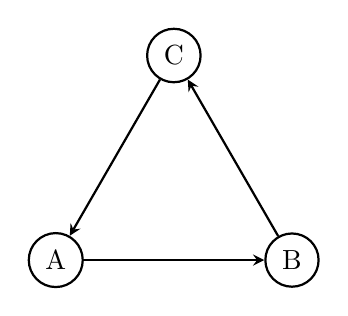
\begin{tikzpicture}[->, >=stealth, thick, scale=1.5]
    % Nodes at triangle vertices
    \node[circle, draw] (A) at (0,0) {A};
    \node[circle, draw] (B) at (2,0) {B};
    \node[circle, draw] (C) at (1,1.732) {C}; % height = sqrt(3)

    % Arrows showing delegation
    \draw (A) -- (B);
    \draw (B) -- (C);
    \draw (C) -- (A);
  \end{tikzpicture}
  \caption{Delegation cycle: A delegates to B, B to C, and C back to A.}
  \label{fig:triangle-cycle}
\end{figure}

This issue is particularly problematic because it can nullify votes without the affected users becoming aware of it. In systems where cycles are not explicitly detected and handled, these votes could be discarded silently, potentially changing the final outcome of the votes.

A simplistic method to prevent cycles is to check whether a delegation would create a cycle before allowing it. For example, if Alice tries to delegate her vote to Bob, the system checks whether Bob has already directly or indirectly delegated their vote to Alice. If so, the delegation is rejected. However, this approach can be cumbersome and may lead to a poor user experience, as users may not understand why their delegation was denied.

Delegation cycles are particularly likely to emerge in dynamic, real-time voting systems like vodle, where users can add, remove, or modify delegations at any time. Even delegation chains that are initially valid may later form part of a cycle as other participants update their preferences. This makes cycle detection not just a one-off validation step, but an ongoing requirement for maintaining consistency and ensuring vote resolution remains reliable.

\subsection*{Abstentions}

A voter abstains by neither casting a vote nor delegating it to another user \citep{brill_liquid_2022}. This includes both deliberate abstention, where a voter knowingly chooses not to participate, and passive abstention, where a voter may be unaware of an ongoing poll or are unable to engage with it.

Abstentions are especially impactful when they occur at the end of a larger delegation chain (see Figure~\ref{fig:delegation-abstention}), as all votes passed along the chain to that voter are effectively lost \citep{brill_liquid_2022}. Additionally, the voters whose decisions were passed along the chain may also be unaware that their votes have been nullified, worsening the effect of the abstention.

\begin{figure}[H]
  \centering
  \begin{tikzpicture}[->, >=stealth, thick, node distance=2.5cm]
    \node[circle, draw] (A) {A};
    \node[circle, draw, right of=A] (B) {B};
    \node[regular polygon, regular polygon sides=3, shape border rotate=0, draw, minimum size=1cm, inner sep=0pt, right of=B] (C) {C};

    \draw (A) -- (B);
    \draw (B) -- (C);
  \end{tikzpicture}
  \caption{Delegation chain ending in abstention: A delegates to B, B to C. C abstains, causing the votes of A and B to be lost.}
  \label{fig:delegation-abstention}
\end{figure}

\subsection*{Super-Voters}
\begin{figure}[H]
  \centering
  \begin{tikzpicture}[->, >=stealth, thick, node distance=2.5cm, square/.style={regular polygon,regular polygon sides=4}]
    \node[circle, draw] (A) {A};
    \node[circle, draw, right of=A] (B) {B};
    \node[square, draw, minimum size=1cm, inner sep=0pt, right of=B] (C) {C};
    \node[square, draw, minimum size=1cm, inner sep=0pt, right of=C] (D) {D};
    \node[square, draw, minimum size=1cm, inner sep=0pt, right of=D] (E) {E};

    \draw (A) -- (B);
    \draw (B) -- (C);
  \end{tikzpicture}
  \caption{Super-voter: A delegates to B, B to C. No matter which vote D or E cast, C's vote will always determine the outcome as it has a weight of 3.}
  \label{fig:delegation-supervoter}
\end{figure}

In liquid democracy, a \textit{super-voter} is a user who receives a large number of delegations, thereby accumulating significant voting power \citep{kling2015votingbehaviourpoweronline}. While such concentration may arise from genuine trust, it risks creating imbalances that contradict the egalitarian goals of the system. Super-voters can effectively act as unelected representatives -- potentially swaying results with little accountability.

Even when systems allow voters to revoke delegations at any time, many users may not actively monitor how their vote is used. This can lead to persistent power structures where a small number of users hold substantial, often unnoticed, influence over outcomes.

This phenomenon is not just theoretical. In the German Pirate Party's use of LiquidFeedback, some participants became so dominant that their votes carried decree-like weight, even though they were not formally elected \citep{sven_becker_liquid_2012, kling2015votingbehaviourpoweronline}. While \citet{kling2015votingbehaviourpoweronline} observed that these super-voters generally aligned with majority opinion, contributing to system stability rather than distorting it, their disproportionate influence still raises concerns about transparency and the extent to which individual voters retain meaningful control over their vote.

Super-voting is not confined to traditional political platforms. In decentralised autonomous organisations (DAOs), which use token-based voting on blockchains, similar patterns emerge. \citet{hallWhatHappensWhen2024} found that in many DAOs, voting power was highly concentrated among a few delegates due to low overall participation. In some cases, such as Gitcoin, over 90\% of votes cast were controlled by the top five delegates.

These examples underscore the importance of delegation mechanisms that can curb excessive power accumulation. Techniques such as weighted delegation and capping the maximum voting power of an individual are essential to preserving fairness, especially in systems like vodle that prioritise inclusivity and trust-based participation.

\subsection{Variations of Liquid Democracy}
This section explores several proposed extensions to liquid democracy that address the limitations outlined above. While many models offer theoretical advantages, particular attention is paid to ranked delegation and weighted delegation -- two techniques that are not only promising from a fairness and robustness perspective, but also feasible to implement within vodle's existing architecture.

The challenges discussed in the previous section, such as delegation cycles, vote loss due to abstentions, and the emergence of super-voters, highlight inherent vulnerabilities in the standard liquid democracy model. To mitigate these issues, enhancements have been proposed that modify how delegations function. These include techniques that allow voters to specify multiple delegates or distribute their vote to multiple casting voters. Each approach introduces different trade-offs and requires algorithmic support to ensure sound and interpretable outcomes.

The following subsections present several such variations, along with the algorithms that can be used to implement them.
\subsection*{Ranked Delegation -- TODO: ADD DIAGRAMS}\label{subsec:background_ranked_delegation}
Ranked delegation improves liquid democracy by allowing voters to list several trusted delegates in order of preference. Instead of choosing just one delegate, a voter can specify a ranked list so that if their top choice is unavailable (e.g. due to abstention or being a part of a delegation cycle) the system can use the next delegate specified.

Implementing ranked delegation requires a mechanism to decide among multiple possible delegation paths -- a route that a vote can take through the delegation graph to reach a casting voter.
This is done through a \textit{delegation rule}, a function that, given a ranked delegation instance and a delegating voter, selects a unique path leading to a \textit{casting voter} \citep{brill_liquid_2022}.

The following key properties help evaluate these delegation rules:

\begin{itemize}
  \item \textbf{Guru Participation:} Ensures that a voter accepting delegated votes (a ``guru'') is never worse off by doing so. Receiving additional delegations should not decrease their influence over the final outcome \citep{kotsialou_riley_2020}. 
  \item \textbf{Confluence:} Guarantees that each delegating voter ends up with one clear and unambiguous delegation path. This property simplifies vote resolution and enhances transparency \citep{brill_liquid_2022}. 
  \item \textbf{Copy Robustness:} Prevents strategic manipulation where a voter might mimic their delegate's vote outside the system to gain extra influence. A copy-robust rule makes sure that duplicating a vote externally does not yield more combined power than a proper delegation \citep{brill_liquid_2022,behrens_2015}. 
\end{itemize}

The literature considers several delegation rules, each with distinct trade-offs:

\textbf{Depth-First Delegation (DFD):} Selects the path beginning with the highest-ranked delegate, even if the resulting chain is long. Although it prioritises individual trust preferences, DFD can violate guru participation \citep{kotsialou_riley_2020}.

\textbf{Breadth-First Delegation (BFD):} Chooses the shortest available delegation path and uses rankings only to resolve ties. This approach usually produces direct, predictable chains and satisfies guru participation, although it might sometimes assign a vote to a lower-ranked delegate \citep{kotsialou_riley_2020, brill_liquid_2022}.

\textbf{MinSum:} Balances path length and delegation quality by selecting the path with the lowest total sum of edge ranks. Due to this, MinSum avoids both unnecessarily long chains and poorly ranked delegations \citep{brill_liquid_2022}.

\textbf{Diffusion:} Constructs delegation paths in stages by assigning votes layer by layer based on the lowest available rank at each step. This method tends to avoid poor delegations but can sometimes produce unintuitive outcomes due to its tie-breaking procedure \citep{brill_liquid_2022}.

\textbf{Leximax:} Compares paths based on their worst-ranked edge. This ensures that especially low-ranked delegations are avoided early in the path while maintaining confluence \citep{brill_liquid_2022}.

\textbf{BordaBranching:} Takes a global view of the delegation graph by selecting a branching that minimises the total rank across all delegation edges. It satisfies both guru participation and copy robustness, though it is more computationally intensive \citep{brill_liquid_2022}.

In summary, ranked delegation enhances liquid democracy by reducing the risk of lost votes. The choice of delegation rule not only affects system efficiency but also influences fairness and robustness. While simpler methods such as DFD and BFD are easier to implement, advanced rules like MinSum, Leximax, and BordaBranching offer stronger guarantees and are better suited for practical deployment in platforms such as vodle.

Based on these considerations, the project adopts the MinSum rule. It offers a clear trade-off between delegation quality, computational efficiency, and user interpretability, making it well-suited for deployment within vodle. By selecting the path with the lowest total rank sum, MinSum prioritises higher-ranked delegates while avoiding unnecessarily long or indirect chains. This supports user trust and clarity by ensuring that final delegation paths reflect stated preferences in an understandable way.


\subsection*{Weighted Delegation -- TODO: ADD DIAGRAMS}\label{subsec:background_weighted_delegation}

Traditional delegation systems, which require voters to delegate their entire vote to a single individual, introduce significant risks such as vote loss through delegate abstentions, delegation cycles, and excessive concentration of voting power in the hands of a few super-voters. To mitigate these issues, weighted delegation allows voters to divide their voting power among multiple delegates, rather than assigning it entirely to one. This approach provides greater flexibility and robustness while preserving voter intent more accurately.

Weighted delegation offers several key advantages:
\begin{itemize}
  \item \textbf{Increased resilience:} Distributing votes across multiple delegates mitigates the effect of abstentions by individual delegates.
  \item \textbf{Reduced concentration of power:} Allowing partial votes to different delegates decreases the likelihood of any single delegate becoming a super-voter.
  \item \textbf{Enhanced voter expression:} Voters can more precisely express their preferences and trust levels by allocating voting power proportionally to multiple individuals.
\end{itemize}

Several methodologies for implementing weighted delegation have been explored in the literature, each with its strengths and weaknesses:

\subsubsection*{Equal Vote Distribution~\citep{degrave2014}}
Degrave's approach allows voters to distribute their votes evenly among multiple delegates. Voters select a group of delegates, and their vote is equally distributed amongst those that do not abstain.
Although this system is intuitive and reduces the impact of abstentions, it lacks flexibility as voters cannot express differing trust levels towards each delegate. Additionally, a critical limitation is the inability for voters to allocate any portion of their vote to themselves, meaning voters are forced to either delegate their entire voting power or none of it, severely limiting personal control over a user's final vote.

\subsubsection{Fractional Delegation~\citep{bersetche2024}}

\citeauthor{bersetche2024} proposes a generalisation of liquid democracy in which voters are allowed to divide their voting weight arbitrarily among multiple delegates, while optionally retaining a fraction for themselves. Each agent expresses their preferences through a delegation matrix, where each entry specifies the proportion of voting weight delegated to a given individual. This approach enables a more flexible expression of trust relationships compared to classical single-delegation models.

To ensure the system remains stable and to prevent cases such as delegation cycles, \citeauthor{bersetche2024} introduces an artificial agent, referred to as agent \(n+1\). Every delegation path carries a small probability (\(\varepsilon\)) of transferring the voting weight to this agent. This mechanism ensures that votes trapped in delegation cycles or excessively long chains are eventually absorbed, preventing them from destabilising the voting process. In the limit as \(\varepsilon \to 0\), the model approximates the classical behaviour of liquid democracy without losses, but with \(\varepsilon > 0\), it guarantees the existence of equilibrium states.

Votes absorbed by agent \(n+1\) are effectively considered lost. As a result, users who delegate without ultimately terminating in a direct voter may see a fraction of their influence dissipate. This diverges from standard liquid democracy approaches, where all delegated votes are ultimately assumed to participate in the outcome.

Overall, fractional delegation as formalised by Bersetche retains desirable properties such as self-selection, delegation consistency, and conservation of total voting weight (accounting for losses), while enabling more expressive delegation structures and guaranteeing equilibrium under mild conditions.


\subsubsection*{Trust Matrix Model (proposed by Heitzig)}

This model was originally proposed by Jobst Heitzig, co-supervisor of this project, as a highly expressive approach to vote splitting within ratings-based voting systems. Rather than directly casting or delegating votes, voters assign trust values \( \text{trust}_{i,j} \in [0, 1] \) to other participants (including themselves), representing the proportion of influence each delegate should have in determining their effective rating. These trust values are used to iteratively compute the final effective rating for each voter.

Let \( \text{rating}_{i,x} \) denote the direct rating that voter \( i \) assigns to option \( x \), and \( \text{eff}_{i,x} \) denote their final effective rating. Then, \( \text{eff}_{i,x} \) can be defined as a combination of the voter's own rating and the effective ratings of their delegates, determined by the trust levels specified:

\begin{gather}
  \text{eff}_{i,x} = \text{trust}_{i,i} \cdot \text{rating}_{i,x} + \sum_{j \neq i} \text{trust}_{i,j} \cdot \text{eff}_{j,x}
\end{gather}

Each voter's trust values must sum to exactly 1:
\[
\sum_{j} \text{trust}_{i,j} = 1
\]

The computation proceeds iteratively, with the effective ratings updated at each step based on the current estimates of delegates' effective ratings. This process continues until there is no longer a change in the effective ratings. Convergence is guaranteed when each voter has some nonzero self-trust (\( \text{trust}_{i,i} > 0 \)), as the system then forms a contraction mapping and Banach's fixed point theorem applies.

% The convergence property can be formalised as follows.

% \paragraph{Convergence Proof.}
% Let there be \( n \) voters and let \( \mathbf{r} = (r_1, \dots, r_n) \in \mathbb{R}^n \) represent the vector of direct ratings for a fixed option, where \( r_i \) is the rating voter \( i \) assigns directly.

% Let \( T \in \mathbb{R}^{n \times n} \) be the \emph{trust matrix}, where \( T_{i,j} \) denotes the proportion of voter \( i \)'s trust allocated to voter \( j \). Assume that each row sums exactly to 1 and that each voter retains some nonzero self-trust (\( T_{i,i} > 0 \)).

% Let \( \mathbf{e}^{(k)} \in \mathbb{R}^n \) denote the vector of effective ratings at iteration \( k \), and define the update rule:
% \[
% \mathbf{e}^{(k+1)} = D \mathbf{r} + A \mathbf{e}^{(k)},
% \]
% where \( D = \text{diag}(T_{1,1}, \dots, T_{n,n}) \) and \( A_{i,j} = T_{i,j} \) for \( i \neq j \), \( A_{i,i} = 0 \).

% Define the function \( f: \mathbb{R}^n \to \mathbb{R}^n \) by \( f(\mathbf{e}) = D \mathbf{r} + A \mathbf{e} \). We observe:
% \[
% \| f(\mathbf{e}) - f(\mathbf{e}') \|_\infty = \| A (\mathbf{e} - \mathbf{e}') \|_\infty \leq \| A \|_\infty \cdot \| \mathbf{e} - \mathbf{e}' \|_\infty,
% \]
% where \( \| A \|_\infty = \max_i \sum_{j} |A_{i,j}| < 1 \) due to the presence of nonzero self-trust.

% Thus, \( f \) is a contraction mapping. By Banach's Fixed-Point Theorem, there exists a unique fixed point \( \mathbf{e}^* \), and the sequence \( (\mathbf{e}^{(k)}) \) converges to \( \mathbf{e}^* \) from any starting point.

% \qed


This model offers the highest granularity and flexibility, allowing voters to finely express confidence across multiple delegates per option. However, it also introduces significant computational overhead and may scale poorly in densely connected delegation graphs. Additionally, users may find it difficult to understand or maintain trust matrices of this complexity, raising potential usability concerns in real-world systems.

\subsubsection*{Summary of Approaches}
% \begin{table}[H]
%   \centering
%   \caption{Comparison of Weighted Delegation Mechanisms}
%   \begin{tabular}{p{3.5cm} p{3.8cm} p{3.5cm} p{3cm}}
%   \hline
%   \textbf{Method} & \textbf{Voter Expressivity} & \textbf{Complexity (Comp. + UI)} & \textbf{Supports Self-Allocation} \\
%   \hline
%   Equal Vote Distribution (Degrave) & Low -- Equal trust across all delegates & Low -- Simple to implement and use & $\times$ \\
%   Fractional Delegation (Bersetche) & Medium -- Explicit per-delegate weights & Medium -- Moderate UI and tracking burden & \checkmark \\
%   Trust Matrix Model (Heitzig) & High -- Nuanced trust relationships among all agents & High -- Requires iterative computation and thoughtful UI design & \checkmark \\
%   \hline
%   \end{tabular}
%   \label{tab:votesplitting}
% \end{table}

\begin{itemize}
  \item \textbf{Equal Vote Distribution (Degrave)} excels in simplicity and ease of implementation, ensuring robustness through straightforward delegation. However, it significantly limits voter expression and prohibits voters from allocating votes to themselves.
  \item \textbf{Fractional Delegation (Bersetche)} provides greater flexibility, permitting detailed voter preference expression, including self-allocation of votes. This method increases both computational complexity and interface complexity.
  \item \textbf{Trust Matrix Model} offers the highest expressivity and detail in delegation relationships, capturing complex trust dynamics. However, this method entails substantial computational overhead and introduces complexity in terms of usability and understanding for voters.
\end{itemize}

Each vote-splitting method balances voter expressivity, computational complexity, and ease of implementation differently. After evaluating these trade-offs, this project selects the trust matrix model for its high expressiveness and compatibility with vodle's principles of autonomy and transparency. While more computationally intensive, it captures nuanced trust relationships and enables fine-grained participation -- both essential for resilient, inclusive decision-making at scale.

\section{Existing Implementations of Liquid Democracy}
To understand how liquid democracy can be integrated into vodle, it is important to examine how similar systems have been implemented in real-world contexts. 
This section explores two implementations, LiquidFeedback and Google Votes, that offer valuable insights into the technical, social, and usability challenges associated with applying liquid democracy at scale.
\subsection{LiquidFeedback}
LiquidFeedback is one of the earliest and most influential real-world implementations of liquid democracy. Developed as an open-source platform, it was notably adopted by the German Pirate Party in 2010 to facilitate internal policy-making through online participation \citep{behrens_liquidfeedback_2014}. The platform allowed members to submit proposals, debate them in structured phases, and vote either directly or via transitive delegation.

In LiquidFeedback, users could choose different delegates for different topics, allowing them to assign their vote to someone they trusted on a specific issue. These choices remained in place until the user changed them, which meant that certain individuals could gradually accumulate more influence if others did not update their delegations. When multiple proposals were put forward, the system used a ranking-based voting method (the Schulze method) to decide which one should win. The Schulze method compares proposals in head-to-head matchups and identifies the option with the strongest overall support, even considering indirect chains of preference. This helped ensure that the winning proposal was broadly supported across the electorate. Importantly, LiquidFeedback only accepted a proposal if it clearly beat the default option of doing nothing, helping to avoid unnecessary or unpopular changes.


In practice, the Pirate Party's use of LiquidFeedback revealed several key dynamics relevant to this project. The platform was successful in enabling large-scale participation and crowd sourced policy formation, but it also demonstrated common risks of liquid democracy. Such as the existence of super-voters, as discussed previously.

Another practical issue was the complexity of the system. LiquidFeedback was difficult to understand for many users, especially those unfamiliar with concepts like transitive delegation or multi-stage voting which limited its accessibility and contributed to declining engagement over time \citep{kling2015votingbehaviourpoweronline}.

For a platform like vodle, the experience of LiquidFeedback highlights several important design considerations. First, user interfaces must be intuitive enough to allow voters to participate without needing deep technical knowledge. Second, the user must know the status of their delegation at a glance - improving the understanding of the platform. Finally, ensuring that votes lead to visible and actionable outcomes is critical for maintaining user engagement.

%Overall, LiquidFeedback serves as both a proof of concept and a cautionary tale; demonstrating that liquid democracy can work at scale, but that thoughtful implementation is essential to avoid replicating the very problems it seeks to solve.
\subsection{Google Votes}
\begin{figure}[H]
  \centering
  \includegraphics[width=0.8\linewidth]{../common/google_votes.png}
  \caption{Screenshot taken from \citet{hardt_google_2015} showing the user interface of Google Votes.}
\end{figure}

Google Votes was an internal experiment at Google designed to explore the practical application of liquid democracy within a corporate environment. Built on top of the company's internal Google+ social network, it operated between 2012 and 2015 and allowed employees to participate in decision making by either voting directly or delegating their vote to a colleague \citep{hardt_google_2015}.

Delegations in Google Votes were category-specific, meaning that users could choose different delegates for different areas of interest, such as food, events, or technical infrastructure. These delegations were persistent but could be overridden at any time, giving users flexibility to either rely on trusted experts or vote independently as needed. The system supported transitive delegation and allowed users to reclaim control by casting their own vote, even after delegating.

The platform placed strong emphasis on usability and transparency. Delegation features were rolled out incrementally, with additional tools such as voting power estimates and delegation advertisements helping users understand their influence. One key design principle was what the authors called the ``Golden Rule of Liquid Democracy'': if a user delegates their vote, they should be able to see how it is being used. To accomplish this, users received notifications when their delegate voted, and all votes were visible to the relevant group. This encouraged accountability and gave voters confidence that their delegated votes were being used appropriately.

While Google Votes was never made publicly available, it served as a successful demonstration of liquid democracy in a structured, real-world setting. It showed that being able to delegate votes could improve engagement and decision making within large organisations, especially when designed with attention to user experience. For vodle, the system provides a concrete example of how features like topic-specific delegation, transparency tools, and real-time voting feedback can make liquid democracy more practical and accessible.
\section{Agent Based Modelling}\label{sec:background_abm}
Agent-based modelling (ABM) is a computational approach used to simulate the actions and interactions of autonomous agents in order to assess their effects on a system as a whole. It is particularly suited for exploring complex, dynamic systems where behaviour emerges from local interactions between individual entities (agents) rather than being dictated by central control. ABM has been widely applied in domains such as economics, sociology, and ecology to study decentralised systems, market dynamics, and collective behaviours \citep{bonabeau2002agent}.

The need to explore ABM arises due to the project's goal of introducing a vote-splitting mechanism that hasn't been explored before into vodle. Traditional analysis alone may not effectively capture the dynamic interactions or unintended consequences that can emerge from this novel feature. Through ABM, it is possible to simulate realistic voting scenarios, track delegation chains, identify potential power imbalances, and anticipate challenges. These simulations can reveal performance insights and inform design decisions before implementing the mechanisms within the live platform.

Several widely used ABM frameworks exist, each with their own strengths and drawbacks relevant to this project:
\begin{itemize}
  \item \textbf{NetLogo} \citep{netlogo} is a highly accessible and widely adopted modelling platform known for its user friendly graphical interface and ease of learning. It offers rapid prototyping capabilities and excellent visualisation features, allowing clear communication of results. However, very complicated models are not compatible with it.
  \item \textbf{Repast} \citep{repast} provides a powerful and versatile suite of tools for building large scale, computationally intensive simulations. It supports distributed computing, which is beneficial for extensive delegation networks with potentially thousands of agents. However, Repast has a steep learning curve, which could hinder its compatibility with this heavily time restricted project.
  \item \textbf{Mesa} \citep{kazil_utilizing_2020} is an open source framework written in Python and specifically designed for agent based modelling. Its advantage lies in its integration with Python's ecosystem of data science libraries. Simulations built with Mesa can easily make use of tools such as NumPy and pandas for efficient data processing, and Matplotlib or Seaborn for visualising model outputs. This compatibility allows for rapid analysis and iteration, while also significantly lowering the learning curve for developers already familiar with Python. Mesa offers a practical balance between usability and computational flexibility, making it well suited for customisable and moderately large simulations.
  \item \textbf{Agents.jl} \citep{agentsjl} is a high-performance agent-based modelling framework written in Julia. Due to Julia's speed and efficiency, it is suitable for large-scale and computationally demanding simulations. The framework is designed to be user-friendly, with a syntax that is approachable for those familiar with scientific computing. However, the Julia ecosystem is less mature compared to Python's, which may limit the availability of additional libraries and resources. However, this trade off may be acceptable for highly performance driven solutions.
\end{itemize}
Given the time constraints of this project, Mesa offers a practical and efficient solution. Its Python-based interface and straightforward setup allow for rapid development without the overhead of learning a new framework. This ease of use enables more time to be spent designing meaningful experiments and analysing results, rather than configuring tooling.
\section{Vodle}
To effectively explore and implement liquid democracy mechanisms, it is essential to understand the design and technical context of the platform into which they are being integrated. Vodle is a web based decision-making tool developed to support participatory group processes through interactive polls and transparent aggregation methods. Its goal is to provide users with flexible, fine grained input mechanisms that encourage compromise between voters, while maintaining accessibility and usability across a broad and diverse user base.

This section introduces the core architecture of vodle, including its underlying rating system (MaxParC) and the technologies that support its operation. These technical foundations were instrumental in shaping the design and feasibility of the advanced delegation features developed in this project.


\subsection{MaxParC}
MaxParC (Maximum Partial Consensus) is the rating system used in vodle to aggregate user preferences and determine poll outcomes. Introduced by \citet{heitzig_fair_2024}, MaxParC was designed to address common limitations of traditional voting systems, particularly the tendency for majority rule to overlook minority preferences. Its goal is to balance fairness, consensus, and efficiency in collective decision making.

In MaxParC, each user rates an option on a scale from $0$ to $100$. This rating reflects the user's willingness to approve that option based on how many other users also support it. Specifically, a rating of $x$ means that the voter will approve the option if fewer than $x\%$ of participants disapprove. A rating of $0$ means the option is never approved, while $100$ means it is always approved regardless of others' opinions. This structure transforms a simple rating into a conditional approval, allowing for a more nuanced expression of preferences with the potential for compromise.

\begin{figure}[H]
  \centering
  \includegraphics[width=0.8\linewidth]{../common/maxparc.png}
  \caption{Visual representation of MaxParC from the perspective of a voter (Alice). Ratings represent conditional approval thresholds. An option is counted as approved by Alice if the approval bar (light grey) overlaps with her rating needle. Graphic from \citet{heitzig_fair_2024}.}
\end{figure}

Understanding how MaxParC processes ratings is essential for this project, as the proposed weighte delegation mechanism must operate within its conditional approval framework. When a user splits their vote among multiple delegates, the system must ensure that their own rating continues to contribute appropriately. Specifically, if a user delegates $x\%$ of their rating to others, their final rating must not fall below $(100-x)\%$ of their original input. This constraint guarantees that the user's approval remains proportionally represented, even when part of their voting power is passed on to others.

Integrating liquid democracy into vodle therefore requires careful design to align with MaxParC's logic, ensuring both technical compatibility and conceptual consistency.

\subsection{Technical Architecture and Implementation Constraints}
Understanding vodle's technology stack is crucial to successfully integrate liquid democracy features into the existing platform. Since the project involves adding complex delegation and voting logic, it's important to appreciate the constraints and benefits of the technologies currently used in vodle, as they directly influence the design and implementation choices.

\subsection*{Angular}
Vodle is built with Angular \citep{angular}, a TypeScript based frontend framework created by Google. Angular's modularity and structured component system provides a strong foundation for incremental development, essential when introducing new features such as ranked delegation that build upon existing components. Its clear separation of concerns helps maintain readable and maintainable code, simplifying debugging and future enhancements. This is particularly beneficial as the delegation logic is expected to grow in complexity and build upon existing components as the project progresses.

\subsection*{Ionic Framework}
The Ionic \citep{ionic} framework complements Angular by enabling the creation of responsive, mobile-compatible applications from a single codebase. Given vodle's goal of broad user participation, Ionic ensures that its functionalities remain consistent and accessible across both desktop and mobile devices. %need to make sure its compatible 
For this project, new delegation features must be designed to work seamlessly within the existing Ionic framework, ensuring that they are visually appealing and user-friendly on all platforms, including mobile devices.

\subsection*{CouchDB}
CouchDB \citep{couchdb} is vodle's primary data storage method and communicates directly with the client through HTTP requests, meaning there is no dedicated backend. This architecture places significant computational responsibilities on the client-side Angular application, including the handling of delegation chains, cycle detection, and the computation of final vote outcomes. Furthermore, since CouchDB stores data exclusively as JSON-formatted strings, complex delegation structures and voting relationships must be serialised and de-serialised on the client side.

The lack of server-side computation means the delegation algorithms must be designed with client-side efficiency in mind, ensuring performance remains acceptable even as delegation complexity increases. Thus, the choice of algorithms for liquid democracy features, such as those to resolve conflicting delegation paths, is directly influenced by CouchDB's architectural constraints.

These technological considerations (covered in more detail in Section~\ref{sec:design_architecture}) strongly shaped the practical implementation of liquid democracy in vodle. They necessitated a focus on efficient client-side logic as well as careful management of data flow.

\subsection{Partially Implemented Delegation in Vodle}\label{subsec:background_existing_delegation}
At the beginning of the project, vodle contained an inactive, partially implemented vote delegation system. Although never deployed in a working state, this prototype included an invitation-based mechanism for initiating delegations, along with early user interface components to support the feature.

However, the implementation lacked several core features required for a robust liquid democracy system. Most notably, it failed to reliably detect or prevent delegation cycles. Since delegation graphs were stored only in each user's local memory, clients could have inconsistent views of the system. This meant delegation actions that appeared valid on one browser could later form a cycle when other users updated their delegations, undermining reliability.

Despite these shortcomings, the incomplete implementation helped clarify key challenges that would need to be addressed in the project. In particular, it highlighted the importance of consistent state synchronisation, clear UI feedback, and reliable validation mechanisms. These lessons informed the redesigned delegation architecture described in Chapter~\ref{ch:design_implementation}.

Further discussion of the issues with this implementation as well as how it was adapted, improved, or replaced can be found in Chapter~\ref{ch:design_implementation}.
% \subsection{Design Philosophy -- TODO}

\section{Summary}
The background research presented in this chapter has provided the necessary foundation for designing and implementing advanced delegation features within vodle. Initially, the research highlighted critical limitations in traditional liquid democracy systems, such as the formation of delegation cycles, the risks associated with abstentions, and the disproportionate influence of super-voters. These insights showed the need for implementing delegation mechanisms that are capable of addressing these challenges effectively.

Research into these mechanisms revealed several promising methods. Ranked delegation was found to be an effective approach for reducing the risk of lost votes, with the MinSum delegation rule being particularly suitable due to its clear balance of efficiency, interpretability, and fairness. Weighted delegation was identified as a valuable strategy to allow voters greater flexibility by distributing their influence among multiple trusted delegates. Additionally, the concept of delegating different options to distinct delegates was supported by practical experiences from Google Votes, where topic-specific delegations improved user engagement and representation accuracy.

Among the weighted delegation methods explored, the trust matrix model stood out for its expressiveness and alignment with vodle's goals of user autonomy and flexibility. By allowing voters to articulate nuanced trust relationships across multiple delegates, including themselves, the model offers a compelling balance between representation quality and individual control. While more computationally intensive than simpler approaches, it presents a viable strategy for robust weighted delegation within a real-time voting system.

The technological constraints of vodle itself, especially the reliance on client-side processing due to the CouchDB architecture, demonstrated the need for efficient, lightweight implementation strategies.

These insights collectively define the project's objectives, which are formalised in the following chapter. The objectives are designed explicitly to address the limitations uncovered in the research, ensuring the integration of liquid democracy into vodle is practical, user-friendly, and aligned with established best practices.